\section{Arbeitsrecht}

\subsection{Verträge auf Arbeitsleistung (Nominatverträge)}

\subsubsection{Arbeitsvertrag}
Arbeitnehmer übernimmt Verpflichtung, Arbeiten gegen Bezahlung für den Arbeitgeber zu verrichten.

\begin{itemize}
    \item Geschuldet ist nicht eine Leistung in Form eines Erfolgs, sondern im Sinne von \underline{sorgfältiges Tätigwerden}.
    \item \textbf{Subordinationsverhältnis}
    \begin{itemize}
        \item Der Arbeitnehmer ordnet sich in persönlicher, betrieblicher, zeitlicher und in gewisser Weise auch in wirtschaftlicher Hinsicht dem Arbeitgeber unter. 
    \end{itemize}
    \item Eingliederung in die Betriebsorganisation
    \begin{itemize}
        \item Arbeitnehmer arbeitet in Büro des Arbeitgebers, trägt die Arbeitskleider, benutzt Arbeitsgeräte welche vom Arbeitgeber bereitgestellt werden etc.
    \end{itemize}
    \item Weitere Kriterien die für das Vorliegen eines Arbeitsverhältnisses sprechen:
    \begin{itemize}
        \item Abführen von Sozialversicherungsbeiträge, Lohnfortzahlung bei Krankheit, fixe oder periodische Entschädigung, wirtschaftliche Abhängigkeit, vertragliche Verpflichtung nicht zu konkurrenzieren
    \end{itemize}
\end{itemize}

\subsubsection{Werkvertrag}
\label{arbeitsrecht:werkvertrag}
Bei einem Werkvertrag verpflichtet sich der Unternehmer, gegen Bezahlung ein Werk für den Besteller herzustellen. Hersteller muss etwas für den Besteller herstellen $\rightarrow$ aktiv sein.

\begin{itemize}
    \item Im Zentrum der Leistung steht das Werk (Bauen eines Hauses, Anfertigen eines Möbelstücks nach den Wünschen des Bestellers, Bauplan eines Ingenieurs, Herstellung eines Massanzugs, ein Haarschnitt).
    \item Es ist der \underline{Erfolg geschuldet}
    \item Unternehmer verwendet i.d.R. eigene Arbeitsmittel
    \item \underline{Einmalige Leistungserbringung}
\end{itemize}

\subsubsection{Auftrag}
\label{arbeitsrecht:auftrag}
Der Beauftragte übernimmt bei einem Auftrag die Verpflichtung, gewisse Geschäfte und Dienste im Interesse des Auftraggebers zu tätigen.

\begin{itemize}
    \item Im Zentrum steht das \underline{sorgfältige Tätigwerden}
    \item Der \underline{Erfolg ist nicht geschuldet}
    \item \underline{Treueverpflichtung} des Beauftragten
    \item Besonderes Vertrauensverhältnis
    \item Selbständige Stellung des Beauftragten
    \item Aufrag ist jederzeit kündbar $\rightarrow$ z.B. wenn Patient kurz vor Operation nicht mehr möchte, kann der Patient nicht dazu gezwungen werden
    \item Beispiel: Dienstleistungen (z.B. Consulting), Erstellen einer Website, etc.
\end{itemize}

\subsection{Rechtsgrundlagen zum Arbeitsrecht}
\textit{Vorrangigkeit der Rechtsgrundlagen:} 

\begin{minipage}{0.5\linewidth} 
    \begin{enumerate}
        \item Bundesverfassung
        \item Gesetze
        \item Verordnungen
        \item Gesamtarbeitsvertrag
        \item Einzelarbeitsvertrag
    \end{enumerate}
\end{minipage}
\begin{minipage}{0.5\linewidth}
    \begin{enumerate}
        \setcounter{enumi}{5}
        \item Normalarbeitsvertrag
        \item Betriebs- und Personalreglemente,\\ Hausordnungen
        \item Weisungen
    \end{enumerate}
\end{minipage}

\subsection{Entstehung eines Arbeitsverhältnisses}

\subsubsection{Einzelarbeitsvertrag}
\begin{itemize}
    \item Grundsätzlich formfrei, Sondervereinbarungen wie Verlängerung der Probezeit, Lohnverzicht bei Überstunden oder Konkurrenzverbot, erfordern aber die schriftliche Form.
    \begin{itemize}
        \item Ein Arbeitsvertrag kann demzufolge auch mündlich oder durch konkludentes Verhalten abgeschlossen werden
        \item \textbf{Beachte}: Das Arbeitsrecht hat diverse \textit{relativ-} und \textit{absolut zwingende Bestimmungen} zum Schutz des Arbeitnehmers.
    \end{itemize}
    \item Übereinstimmende gegenseitige Willenserklärung
    \begin{itemize}
        \item Einigung betreffend Hauptpunkte (Parteien, Beginn und Dauer, Umfang, Arbeitsort, Lohn, Arbeitszeit und Ferien, Probezeit, Kündigungsfrist)
    \end{itemize}
    \item Handlungsfähigkeit der Parteien (Urteilsfähigkeit und Mündigkeit)
    \item Keinen nichtigen Vertragsinhalt (nicht sittenwidrig, widerrechtlich oder unmöglich)
\end{itemize}

\subsubsection{Besondere Einzelarbeitsverträge}
\begin{itemize}
    \item Lehrvertrag, Handelsreisender Vertrag, Heimarbeitsvertrag
\end{itemize}

\subsubsection{Gesamtarbeitsvertrag (GAV)}
\begin{center}
    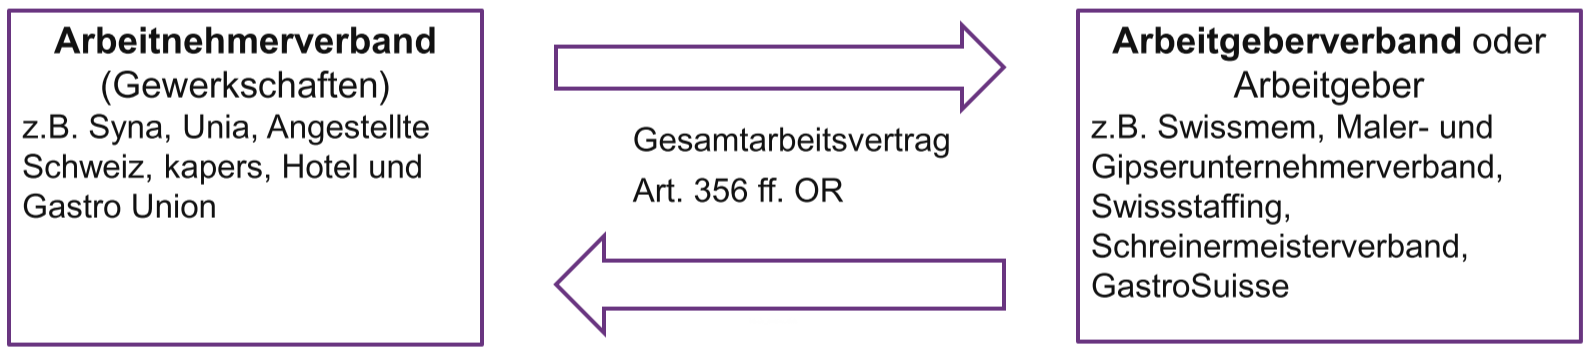
\includegraphics[width=0.6\linewidth]{04-arbeitsrecht/01-gav}
\end{center}

\begin{itemize}
    \item Einfache Schriftlichkeit
    \item Der GAV ist ein Vertrag zwischen \textcolor{OSTPink}{Arbeitgebern} oder \textcolor{OSTPink}{Arbeitgeberverbänden} und \textcolor{OSTPink}{Arbeitnehmerverbänden} zur Regelung der Arbeitsbedingungen zwischen den GAV-Parteien.
    \item Im GAV werden Bestimmungen über Abschluss, Inhalt und Beendigung der einzelnen Arbeitsverhältnisse der beteiligten Arbeitnehmer und Arbeitgeber verhandelt und vereinbart.
\end{itemize}

\subsubsection{Normalarbeitsvertrag (NAV)}
\begin{itemize}
    \item Behördlicher Erlass mit arbeitsvertraglichen Bestimmungen. Diese können zwingenden oder empfehlenden Charakter haben.
    \item \textit{Zwei Arten}: NAV mit \underline{zwingenden Mindestlöhnen} und NAV mit \underline{Bestimmungen über das Arbeitsverhältnis}
    \begin{itemize}
        \item Z.B. Der Bundesrat hat den Normalarbeitsvertrag für Arbeitnehmerinnen und Arbeitnehmer in der Hauswirtschaft (NAV Hauswirtschaft) verabschiedet. Er regelt den Mindestlohn für Hausangestellte in Privathaushalten.
    \end{itemize}
\end{itemize}

\newpage

\subsection{Pflichten Arbeitnehmner}
\begin{itemize}
    \item Der Arbeitnehmer hat die vertraglich übernommene Arbeit in eigener Person zu leisten, sofern nichts anderes verabredet ist oder sich aus den Umständen ergibt.
    \item Befolgung von Anordnungen und Weisungen
    \begin{itemize}
        \item Der Arbeitgeber kann über die Ausführung der Arbeit und das Verhalten der Arbeitnehmer im Betrieb oder Haushalt allgemeine Anordnungen erlassen und ihnen besondere Weisungen erteilen.
    \end{itemize}
    \item \textbf{Sorgfalts- und Treuepflicht}
    \begin{itemize}
        \item Allgemeine Treue- und Sorgfaltspflicht
        \begin{itemize}
            \item Sorgfältige Ausführung der Arbeiten
            \item Handeln nach Treu und Glauben im Interesse des Arbeitgebers (z.B. wenn MA vergisst Alarmanlage am Abend einzuschalten)
        \end{itemize}
        \item Sorgfältiger und fachgerechter Umgang mit Maschinen, Arbeitsgeräten, technischen Einrichtungen und Anlagen sowie Fahrzeugen des Arbeitgebers
        \begin{itemize}
            \item z.B. Kaffee über Laptop leeren
        \end{itemize}
        \item Keine konkurrenzierende- oder treue- und sorgfaltspflichtverletzende Tätigkeiten während der Dauer des Arbeitsverhältnisses
        \begin{itemize}
            \item Konkurrenzierung des Arbeitgebers (Aussendienstmitarbeiter bei AXA (60\%) und bei Mobiliar (40\%) $\rightarrow$ geht nicht, da AXA \& Mobiliar Konkurrenten sind!)
            \item Herabsetzung der Leistungsfähigkeit
            \item Beeinträchtigung des Ansehens des Arbeitgebers
        \end{itemize}
    \end{itemize}
    \item \textbf{Geheimhaltung von Fabrikations- und Geschäftsgeheimnissen}
    \begin{itemize}
        \item Unter Umständen auch für die Zeit nach Beendigung des Arbeitsverhältnisses
        \item Tatsachen gelten als geheim, wenn sie:
        \begin{itemize}
            \item diese \underline{weder offenkundig} noch \underline{allgemein zugänglich} sind und
            \item an deren Geheimhaltung der Arbeitgeber (Geheimnisherr) ein \underline{berechtigtes Interesse} hat und
            \item diese \underline{geheim halten will}.
            \item chliesslich muss das Geheimnis einen \underline{Bezug zum Unternehmen} (Fabrikation oder Geschäft) aufweisen.
        \end{itemize}
        \item Die Gesetzesbestimmung zum Schutz von Geschäftsgeheimnissen ist \underline{offen formuliert}, was zu Rechtsunsicherheiten führen kann. Um sicher zu gehen, sollten daher Geschäftsgeheimnisse explizit als solche gekennzeichnet werden und für jedermann identifizierbar sein.
    \end{itemize}
\end{itemize}

\subsection{Nachträgliches Konkurrenzverbot}
\begin{itemize}
    \item Vertragsklausel, die es dem Arbeitnehmer verbietet nach Beendigung des Arbeitsverhältnisses, für einen Dritten oder selbstständig seine Arbeitgeberin zu konkurrenzieren.
    \item Voraussetzung für ein gültiges Konkurrenzverbot:
    \begin{itemize}
        \item \textbf{Handlungsfähigkeit} des Arbeitnehmers
        \item \textbf{Schriftliche Vereinbarung} (Unterschrift des Arbeitnehmers)
        \item \textbf{Konkurrenzierende Tätigkeit} (gleichartige Leistungen)
        \item \textbf{Einblick in den Kundenkreis} (Aussendienstmitarbeiter) oder in \textbf{Fabrikations- und Geschäftsgeheimnisse} (Kenntnisse über Rezepturen)
        \item \textbf{Erhebliches Schädigungspotenzial} für die Arbeitgeberin (die Kenntnisse selbst müssen dieses Potenzial haben)
        \item \textbf{Angemessene Begrenzung} nach Ort (Geschäftsbereich der Arbeitgeberin), Zeit (i.d.R. nicht mehr als drei Jahre) und Gegenstand
    \end{itemize}
\end{itemize}

\subsubsection{Haftung des Arbeitnehmers aus Vertragsverletzung}
\begin{itemize}
    \item Der Arbeitnehmer ist für den Schaden verantwortlich, den er \underline{absichtlich} oder \underline{fahrlässig} dem Arbeitgeber zufügt.
    \item Das \underline{Mass der Sorgfalt}, für die der Arbeitnehmer einzustehen hat, bestimmt sich nach dem einzelnen Arbeitsverhältnis, unter Berücksichtigung des Berufsrisikos, des Bildungsgrades oder der Fachkenntnisse, die zu der Arbeit verlangt werden, sowie der Fähigkeiten und Eigenschaften des Arbeitnehmers, die der Arbeitgeber gekannt hat oder hätte kennen sollen.
\end{itemize}

Damit ein Arbeitnehmer schadenersatzpflichtig wird, müssen \textbf{vier Voraussetzungen} kumulativ erfüllt sein:
\begin{itemize}
    \item \textbf{Vorliegen eines Schadens}
    \begin{itemize}
        \item Muss Arbeitgeber beweisen
    \end{itemize}
    \item \textbf{Vertragsverletzung des Arbeitnehmers} (Verletzungen von Arbeits-, Sorgfalts- und Treuepflichten)
    \begin{itemize}
        \item Muss Arbeitgeber beweisen
    \end{itemize}
    \item \textbf{Adäquater Kausalzusammenhang} zwischen Schaden und Vertragsverletzung
    \begin{itemize}
        \item uss Arbeitgeber beweisen
    \end{itemize}
    \item \textbf{Verschulden des Arbeitnehmers}
    \begin{itemize}
        \item Wird vermutet, Arbeitnehmer kann sich exkulpieren
        \item Das Verschuldensmass muss in der Praxis vom Arbeitgeber dargelegt werden
    \end{itemize}
\end{itemize}

Grundsätzlich haftet der Arbeitnehmer für jeden Schaden, den er dem Arbeitgeber \underline{absichtlich} oder \underline{fahrlässig} zufügt. Die Haftung des Arbeitnehmers beurteilt sich immer nach dem \underline{konkreten Einzelfall}.\\

Wenn Material durch Verschleiss kaputt geht, kann der Arbeitgeber nicht die Kosten dafür vom Arbeitnehmer verlangen.
Vor allem bei Aushilfsjobs wenn Arbeitnehmer nicht eine entsprechende Qualifikation dafür hat, kann der Arbeitnehmer nicht zur Rechenschaft gezogen werden!

\subsubsection{Faustregeln für Haftungs- und Sorgfaltsmassstab}
\begin{itemize}
    \item \textbf{Absicht}: Schaden ist mit voller Absicht geschehen oder in Kauf genommen worden.
    \begin{itemize}
        \item Schadenersatzpflicht in voller Höhe
    \end{itemize}
    \item \textbf{Grobe Fahrlässigkeit}: Das darf einfach nicht passieren. Wie kann man nur.
    \begin{itemize}
        \item Grundsätzlich keine Reduktion, oft aber maximal 3 Monatslöhne
    \end{itemize}
    \item \textbf{Mittlere Fahrlässigkeit}: So etwas sollte eigentlich nicht passieren.
    \begin{itemize}
        \item Hälfte bis 2 /3 des Schadens, maximal 2 Monatslöhne
    \end{itemize}
    \item \textbf{Leichte Fahrlässigkeit}: Das kann zwar schon einmal passieren, aber man hätte besser aufpassen können.
    \begin{itemize}
        \item Bis zur Hälfte des Schadens, maximal 1 Monatslohn
    \end{itemize}
    \item \textbf{Bagatellfälle}: Das bringt die Arbeit schon einmal mit sich.
    \begin{itemize}
        \item Keine Schadenersatzpflicht
    \end{itemize}
\end{itemize}

\newpage

\subsubsection{Überstundenarbeit}
\begin{itemize}
    \item Wird gegenüber dem zeitlichen Umfang der Arbeit, der verabredet oder üblich oder durch Normalarbeitsvertrag oder Gesamtarbeitsvertrag bestimmt ist, die Leistung von Überstundenarbeit \underline{notwendig}, so ist der Arbeitnehmer dazu soweit verpflichtet, als er sie zu \underline{leisten vermag} und sie ihm nach Treu und Glauben \underline{zugemutet} werden kann. (Zwingende Bestimmung)
    \item Im Einverständnis mit dem Arbeitnehmer kann der Arbeitgeber die Überstundenarbeit innert eines angemessenen Zeitraumes durch \underline{Freizeit von mindestens gleicher Dauer} ausgleichen. (Dispositive Bestimmung)
    \item Wird die Überstundenarbeit nicht durch Freizeit ausgeglichen und ist nichts anderes schriftlich verabredet oder durch Normalarbeitsvertrag oder Gesamtarbeitsvertrag bestimmt, so hat der Arbeitgeber für die Überstundenarbeit Lohn zu entrichten, der sich nach dem Normallohn \underline{samt einem Zuschlag von} \underline{mindestens einem Viertel} bemisst. (Dispositive Bestimmung)
\end{itemize}

\begin{center}
    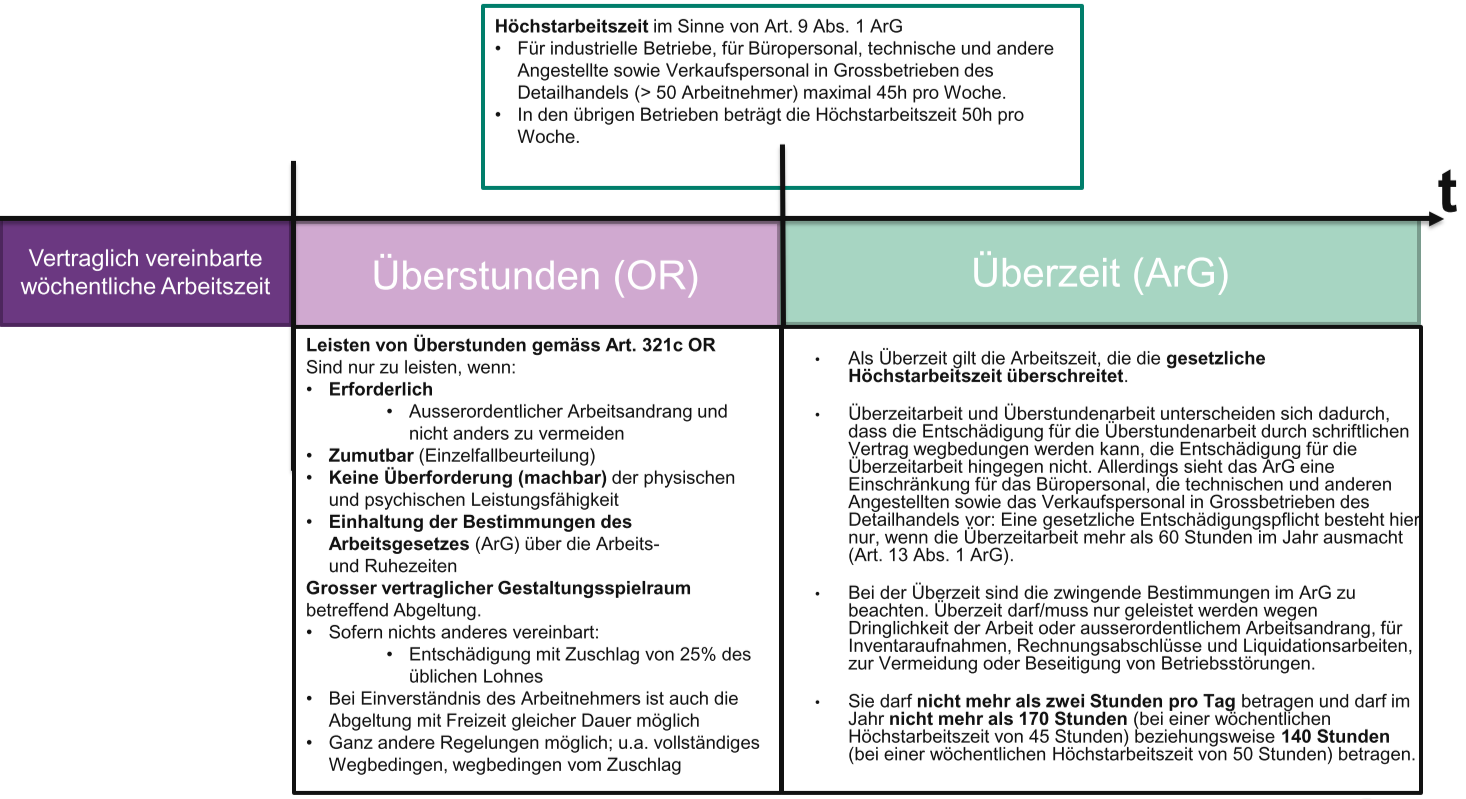
\includegraphics[width=\linewidth]{04-arbeitsrecht/02-ueberstunden}
\end{center}

\subsection{Pflichten Arbeitgeber}
\begin{itemize}
    \item Der Arbeitgeber hat dem Arbeitnehmer den Lohn zu entrichten, der \underline{verabredet} oder \underline{üblich} oder durch \underline{Normalarbeitsvertrag} oder \underline{Gesamtarbeitsvertrag} bestimmt ist.
    \item Sind nicht kürzere Fristen oder andere Termine verabredet oder üblich und ist durch Normalarbeitsvertrag oder Gesamtarbeitsvertrag nichts anderes bestimmt, so ist dem Arbeitnehmer der Lohn \underline{Ende jedes Monats} auszurichten.
\end{itemize}

\subsubsection{Lohnarten}
\begin{minipage}{0.5\linewidth}
    \begin{itemize}
        \item Stundenlohn, Fixlohn, Akkordlohn
        \item Anteil am Geschäftsergebnis
        \item Individuelle Erfolgsbeteiligung
        \item Provision
        \item Gratifikation (Sondervergütung, die bei besonderen Anlässen ausgerichtet wird)
    \end{itemize}
\end{minipage}
\begin{minipage}{0.5\linewidth}
    \begin{itemize}
        \setcounter{enumi}{4}
        \item Naturallohn (Kost und Logis)
        \item Lohnzulagen (Überstundenentschädigung, Nacht- und Sonntagsarbeitszuschläge, Schichtzulagen, Feiertags- und Ferienvergütungen)
        \item Fringe Benefits (Vergünstigungen, Repräsentationsspesen, Clubmitgliedschaften etc.)
    \end{itemize}
\end{minipage}

\subsubsection{Lohn bei Verhinderung des Arbeitnehmers}

\textit{Ohne eigenes Verschulden}
\begin{itemize}
    \item Ohne Verschulden:
    \begin{itemize}
        \item Verkehrsunfälle, «normale» Sportunfälle (Skifahren, Bergsteigen, Tauchen, Reiten oder Deltasegeln Schwangerschaftsabbrüche)
    \end{itemize}
    \item Mit Verschulden:
    \begin{itemize}
        \item Waghalsige Unternehmen wie Fahren in angetrunkenem Zustand, Risikosportarten wie MotocrossRennen, Skitouren trotz grosser Lawinengefahr, Klettertouren trotz drohendem Wettereinbruch, usw.)
    \end{itemize}
\end{itemize}

\textit{Dauer des Arbeitsverhältnisses}
\begin{itemize}
    \item Befristetes AV: Ist für eine gewisse Zeit und \underline{für länger als drei Monate eingegangen} worden.
    \item Unbefristet AV: Ist für unbestimmte Zeit eingegangen und \underline{hat bereits drei Monate gedauert}.
\end{itemize}

\textit{Dauer der Lohnfortzahlung}
\begin{itemize}
    \item Im ersten Dienstjahr drei Wochen
    \item Danach für eine angemessene Zeit gemäss Berner-, Basler- oder Zürcher Skala
    \item Lohnfortzahlung \underline{entsteht in jedem Dienstjahr von neuem}.
    \item Der Anspruch besteht nicht pro Krankheitsereignis, sondern gesamthaft nur einmal pro Dienstjahr. Die verschiedenen Gründe für Abwesenheiten vom Arbeitsplatz werden zusammengezählt.
    \item Der Anspruch besteht bei \underline{teilweiser Verhinderung} an der Arbeit nicht für eine bestimmte Zeit, sondern verlängert sich, bis der Anspruch auf die \underline{volle Lohnfortzahlung} abgegolten ist.
\end{itemize}

\subsubsection{Arbeitszeugniss}
\begin{itemize}
    \item Der Arbeitnehmer kann \textbf{jederzeit} vom Arbeitgeber ein Zeugnis verlangen, das sich über die \underline{Art} und \underline{Dauer} des Arbeitsverhältnisses sowie über seine \underline{Leistungen} und sein \underline{Verhalten} ausspricht.
    \item Ein Vollzeugnis sollte folgende Angaben enthalten:
    \begin{itemize}
        \item \textbf{Identität} des Arbeitnehmers und des Arbeitgebers,
        \item \textbf{Beginn} und \textbf{Ende} des Arbeitsverhältnisses,
        \item detaillierte Auflistung der \textbf{wichtigen Funktionen} und der das Arbeitsverhältnis prägenden Tätigkeiten des Arbeitnehmers und deren \textbf{Zeitdauer},
        \item aussagekräftige \textbf{Bewertung der Leistung} (Arbeitsqualität und -quantität) des Arbeitnehmers und seines Verhaltens,
        \item die rechtsgültige \textbf{Unterschrift} des Arbeitgebers
    \end{itemize}
    \item muss wahrheitsgetreu mit wohlwollender Formulierung sein
\end{itemize}

\subsection{Beendigung des Arbeitsverhältnisses}
\begin{minipage}{0.5\linewidth}
    \begin{itemize}
        \item Kündigung des unbefristeten Einzelarbeitsvertrags
        \item Zeitablauf beim befristeten Einzelarbeitsvertrag
        \item Aufhebungsvertrag
    \end{itemize}
\end{minipage}
\begin{minipage}{0.5\linewidth}
    \begin{itemize}
        \setcounter{enumi}{4}
        \item Fristlose Kündigung
        \item Tod des Arbeitnehmers
        \item Beachte: Nicht der Konkurs des Arbeitsgebers
    \end{itemize}
\end{minipage}

\subsubsection{Kündigung}
\begin{itemize}
    \item Die Vertragsparteien können das Arbeitsverhältnis unter Einhaltung der vertraglichen oder gesetzlichen Frist auflösen, \underline{ohne} dass es einen \underline{besonderen Grund} dafür braucht (Kündigungsfreieheit).
    \begin{itemize}
        \item Kündigungsgrund: schlechte Leistung, wenig Einsatz, viele Fehler, etc
    \end{itemize}
    \item Eine Kündigung ist eine \underline{einseitig, empfangsbedürftige Willenskundgabe}.
    \item Gilt für die Beendigung des Arbeitsverhältnisses ein Endtermin, wie das Ende eines Monats, muss die Kündigung am letzten Tag dieses Monats der Gegenseite \underline{zur Kenntnis gebracht werden}, und nicht erst versendet worden sein.
    \item Kündigung ist \underline{formfrei} möglich, sofern nicht anderst im Arbeitsvertrag geregelt.
\end{itemize}

\paragraph{Kündigung WÄHREND der Probezeit}
\begin{itemize}
    \item erster Monat eines unbefristeten Arbeitsverhältnisses giltet als Probezeit
    \item gibt in Probezeit \underline{keinen} Kündigungsschutz, Arbeitsverhältnis von beiden Parteien \underline{jederzeit} kündbar
    \item Sofern nichts anderes vereinbart beträgt die \textbf{Kündigungsfrist innerhalb der Probezeit 7 Kalendertage}.
    \item Verlängerung der Probezeit \underline{nur} bei Krankheit, Unfall oder einer nicht freiwillig übernommenen gesetzlichen Pflicht möglich
\end{itemize}

\paragraph{Probezeit}
\begin{center}
    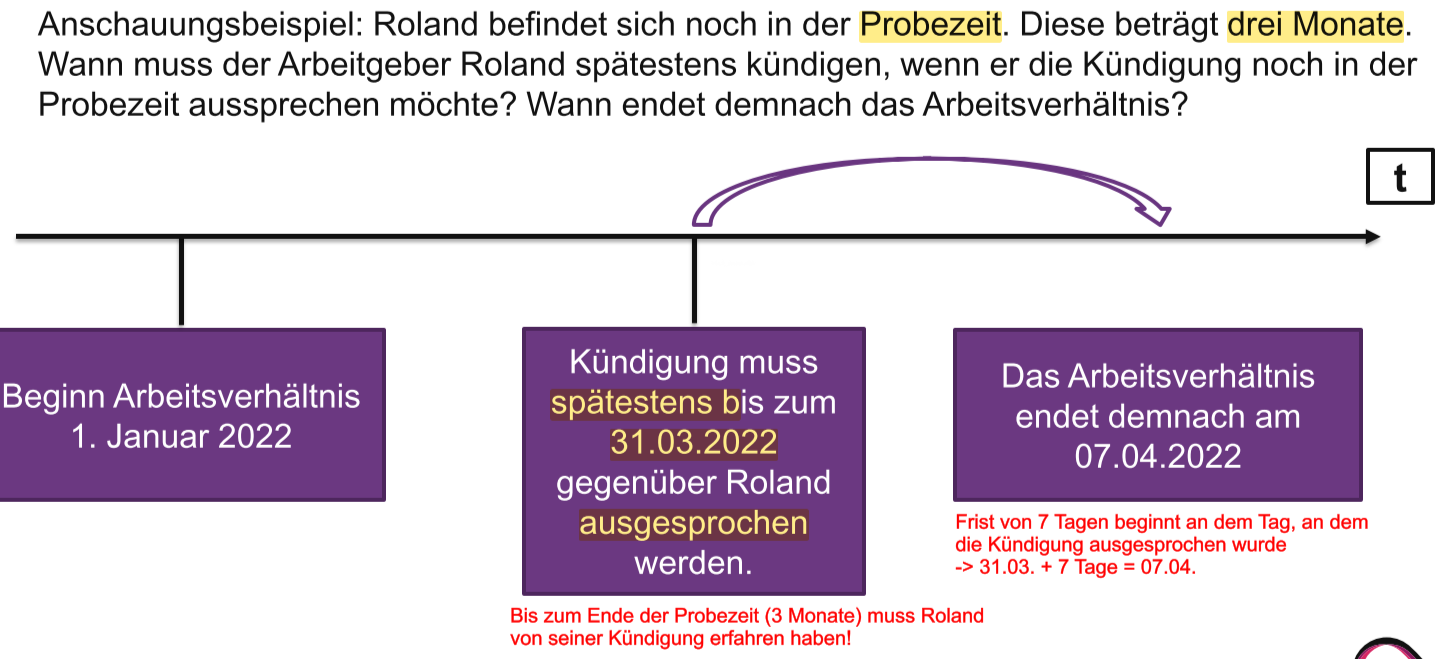
\includegraphics[width=\linewidth]{04-arbeitsrecht/03-probezeit}
\end{center}

\paragraph{Kündigung NACH Probezeit}
\begin{itemize}
    \item Wenn nichts anderes vereinbart worden ist, gelten folgende Kündigungsfristen
    \begin{itemize}
        \item im 1. Dienstjahr $\rightarrow$ 1 Monat
        \item im 2. bis zum 9. Dienstjahr $\rightarrow$ 2 Monate
        \item Ab dem 10. Dienstjahr $\rightarrow$ 3 Monate
        \item Sind nicht zwingend, gelten aber wenn nichts anderes abgemacht/ vereinbart wurde
    \end{itemize}
    \item Durch schriftliche Abrede können andere aber nicht unterschiedliche Fristen vereinbart werden.
\end{itemize}

\subsubsection{Missbräuchliche Kündigung}
\begin{itemize}
    \item Kündigen wegen gewisser religiöser Ausrichtung
    \item Kündigung des Arbeitnehmers nach 44 Dienstjahren kurz vor Erreichung des Pensionsanspruchs und ohne zureichende Gründe
    \item Rachekündigung: Einem Arbeitnehmer wird gekündigt, weil er ein ihm zustehendes Recht geltend macht.
\end{itemize}

Wer die Missbräuchlichkeit einer Kündigung geltend machen will, muss zwei Fristen zwingend einhalten, die \textbf{Einsprachefrist} (bis zum Ablauf der Kündigungsfrist) und die \textbf{Klagefrist} (180 Tage nach Beendigung des
Arbeitsverhältnisses).

\begin{center}
    \includegraphics[width=\linewidth]{04-arbeitsrecht/04-kündigungsfrist}
\end{center}

\paragraph{Rechtsfolgen missbräuchlicher Kündigung}
\begin{itemize}
    \item Selbst wenn das Gericht eine Kündigung als missbräuchlich qualifiziert, ist diese \underline{rechtswirksam}.
    \item Der Arbeitnehmer hat aber Anspruch auf eine \textbf{Entschädigungszahlung}. Diese beträgt \underline{maximal sechs Monatslöhne}, wobei die Festlegung der Höhe der Entschädigung im Ermessen des Richters liegt.
\end{itemize}

\subsubsection{Kündigung zur Unzeit}
\begin{itemize}
    \item Insbesondere bei Arbeitsverhinderungen infolge Krankheit und Unfall, bei Schwangerschaft und Mutterschaft sowie bei Dienstleistungen für Hilfsaktionen im Ausland besteht aber ein \underline{zeitlich begrenzter Kündigungsschutz}
    \begin{itemize}
        \item \textit{Zeitlicher Kündigungsschutz giltet nur, wenn die Probezeit angelaufen ist und der Arbeitgeber die Kündigung ausgesprochen hat!!!}
    \end{itemize}
    \item Der Kündigungsschutz kommt mit gleicher Dauer auch bei Teilzeit- und Temporärarbeitsverhältnissen sowie grundsätzlich bei Freistellung zum Tragen. \underline{Keine Anwendung} findet der Kündigungsschutz bei befristeten Arbeitsverhältnissen, Aufhebungsverträgen und bei fristlosen Entlassungen (zumindest bei gerechtfertigten).
    \item \textbf{Merke}: Die Sperrfrist resp. der Kündigungsschutz gilt erst \underline{nach Ablauf der Probezeit} und nur bei einer \underline{Arbeitgeberkündigung}
\end{itemize}

\paragraph{Sperrfristen}
\begin{itemize}
    \item Bei obligatorischem schweizerischen Militärdienst, Zivilschutz, Zivildienst \textbf{4 Wochen vor und 4 Wochen nach} der Dienstleistung, sofern diese \underline{mehr als 11 Tage dauert} und während der Zeit der Dienstleistung
    \item Bei Krankheit oder Unfall
    \begin{itemize}
        \item 30 Tage im 1. Dienstjahr
        \item 90 Tage vom 2. bis und mit 5. Dienstjahr
        \item 180 Tage ab dem 6. Dienstjahr
    \end{itemize}
    \item Bei Schwangerschaft und Niederkunft während der \underline{ganzen Dauer} der Schwangerschaft \underline{bis und mit sechzehn Wochen} nach der Geburt
    \item Bei Dienstleistungen für Hilfsaktionen im Ausland für die \underline{Dauer der Dienstleistung}
    \item \textbf{Merke}: Die Anwendung der Sperrfristen hat mit der Lohnfortzahlungspflicht des Arbeitgebers bei Arbeitsverhinderung nichts zu tun.
\end{itemize}

\begin{center}
    \includegraphics[width=0.95\linewidth]{04-arbeitsrecht/05-kündigung_unzeit}
\end{center}

\subsubsection{Ausserordentliche Kündigung}
\begin{itemize}
    \item Aus wichtigen Gründen kann der Arbeitgeber wie der Arbeitnehmer \underline{jederzeit} das Arbeitsverhältnis \underline{fristlos} auflösen; er muss die fristlose Vertragsauflösung schriftlich begründen, wenn die andere Partei dies verlangt.
    \item Als wichtiger Grund gilt namentlich jeder Umstand, bei dessen Vorhandensein dem Kündigenden nach Treu und Glauben die \underline{Fortsetzung des Arbeitsverhältnisses nicht mehr zugemutet} werden darf. (Vertrauensverhältnis ist zerrüttet)
    \item Über das Vorhandensein solcher Umstände entscheidet der Richter nach seinem \underline{Ermessen}, darf aber in keinem Fall die unverschuldete Verhinderung des Arbeitnehmers an der Arbeitsleistung als wichtigen Grund anerkennen.
    \item \textbf{Merke}: Die fristlose Auflösung ist ein Notventil und wird daher in der Gerichtspraxis nur dann geschützt, wenn der Anlass zur Kündigung ausreichend gravierend ist.
    \item Liegt der wichtige Grund zur fristlosen Auflösung des Arbeitsverhältnisses im vertragswidrigen Verhalten einer Vertragspartei, so hat diese \underline{vollen Schadenersatz} zu leisten, \underline{unter Berücksichtigung aller aus dem Arbeitsverhältnis entstehenden Forderungen}.
\end{itemize}

\subsection{Rechte an Erfindungen und Designs}
\begin{itemize}
    \item Die Grenze liegt dort, wo ein Mitarbeiter \underline{selbständig, kreativ und schöpferisch} tätig wird.
    \item Erfindung: wenn dank einer schöpferischen Idee durch eine neue, originelle Kombination von Naturkräften oder -stoffen ein technischer Nutzeffekt erzielt wird, der einen wesentlichen technischen Fortschritt bedeutet.
    \item Designs sind Gestaltungen von Erzeugnissen oder Teilen von Erzeugnissen, die namentlich durch die Anordnung von Linien, Flächen, Konturen oder Farben oder durch das verwendete Material charakterisiert sind.
\end{itemize}

\paragraph{Dienst- oder Aufgabenerfindungen}
\begin{itemize}
    \item Das sind Erfindungen oder Designs, welche erstens in Ausübung der dienstlichen Tätigkeit und zweitens in Erfüllung der arbeitsvertraglichen Pflichten entstanden sind.
    \item gehören dem Auftraggeber, sofern nichts anderes Vereinbart wurde
    \item Gelegenheitserfindungen (entsteht zufällig \& gehört \underline{nicht} zum Auftragsgebiet), steht diese dem Arbeitnehmer zu
\end{itemize}